%%%%%%%%%%%%%%%%%%%%%%%%%%%%%%%%%%%%%%%%%%%%%%%%%%%%%%%%%%%%%%%
%% BRIEF VERSION OF OXFORD THESIS TEMPLATE FOR CHAPTER PREVIEWS

%%%%% CHOOSE PAGE LAYOUT
% format for PDF output (ie equal margins, no extra blank pages):
\documentclass[a4paper,nobind]{templates/ociamthesis}

% UL 5 January 2021 - add packages used by kableExtra
\usepackage{booktabs}
\usepackage{longtable}
\usepackage{array}
\usepackage{multirow}
\usepackage{wrapfig}
\usepackage{colortbl}
\usepackage{pdflscape}
\usepackage{tabu}
\usepackage{threeparttable}
\usepackage{threeparttablex}
\usepackage[normalem]{ulem}
\usepackage{makecell}
\usepackage[colorlinks=false,pdfpagelabels,hidelinks=]{hyperref}
\usepackage{float}


%UL set section header spacing
\usepackage{titlesec}
% 
\titlespacing\subsubsection{0pt}{24pt plus 4pt minus 2pt}{0pt plus 2pt minus 2pt}

% UL 30 Nov 2018 pandoc puts lists in 'tightlist' command when no space between bullet points in Rmd file
\providecommand{\tightlist}{%
  \setlength{\itemsep}{0pt}\setlength{\parskip}{0pt}}
 
% UL 1 Dec 2018, fix to include code in shaded environments
\usepackage{color}
\usepackage{fancyvrb}
\newcommand{\VerbBar}{|}
\newcommand{\VERB}{\Verb[commandchars=\\\{\}]}
\DefineVerbatimEnvironment{Highlighting}{Verbatim}{commandchars=\\\{\}}
% Add ',fontsize=\small' for more characters per line
\usepackage{framed}
\definecolor{shadecolor}{RGB}{248,248,248}
\newenvironment{Shaded}{\begin{snugshade}}{\end{snugshade}}
\newcommand{\AlertTok}[1]{\textcolor[rgb]{0.94,0.16,0.16}{#1}}
\newcommand{\AnnotationTok}[1]{\textcolor[rgb]{0.56,0.35,0.01}{\textbf{\textit{#1}}}}
\newcommand{\AttributeTok}[1]{\textcolor[rgb]{0.77,0.63,0.00}{#1}}
\newcommand{\BaseNTok}[1]{\textcolor[rgb]{0.00,0.00,0.81}{#1}}
\newcommand{\BuiltInTok}[1]{#1}
\newcommand{\CharTok}[1]{\textcolor[rgb]{0.31,0.60,0.02}{#1}}
\newcommand{\CommentTok}[1]{\textcolor[rgb]{0.56,0.35,0.01}{\textit{#1}}}
\newcommand{\CommentVarTok}[1]{\textcolor[rgb]{0.56,0.35,0.01}{\textbf{\textit{#1}}}}
\newcommand{\ConstantTok}[1]{\textcolor[rgb]{0.00,0.00,0.00}{#1}}
\newcommand{\ControlFlowTok}[1]{\textcolor[rgb]{0.13,0.29,0.53}{\textbf{#1}}}
\newcommand{\DataTypeTok}[1]{\textcolor[rgb]{0.13,0.29,0.53}{#1}}
\newcommand{\DecValTok}[1]{\textcolor[rgb]{0.00,0.00,0.81}{#1}}
\newcommand{\DocumentationTok}[1]{\textcolor[rgb]{0.56,0.35,0.01}{\textbf{\textit{#1}}}}
\newcommand{\ErrorTok}[1]{\textcolor[rgb]{0.64,0.00,0.00}{\textbf{#1}}}
\newcommand{\ExtensionTok}[1]{#1}
\newcommand{\FloatTok}[1]{\textcolor[rgb]{0.00,0.00,0.81}{#1}}
\newcommand{\FunctionTok}[1]{\textcolor[rgb]{0.00,0.00,0.00}{#1}}
\newcommand{\ImportTok}[1]{#1}
\newcommand{\InformationTok}[1]{\textcolor[rgb]{0.56,0.35,0.01}{\textbf{\textit{#1}}}}
\newcommand{\KeywordTok}[1]{\textcolor[rgb]{0.13,0.29,0.53}{\textbf{#1}}}
\newcommand{\NormalTok}[1]{#1}
\newcommand{\OperatorTok}[1]{\textcolor[rgb]{0.81,0.36,0.00}{\textbf{#1}}}
\newcommand{\OtherTok}[1]{\textcolor[rgb]{0.56,0.35,0.01}{#1}}
\newcommand{\PreprocessorTok}[1]{\textcolor[rgb]{0.56,0.35,0.01}{\textit{#1}}}
\newcommand{\RegionMarkerTok}[1]{#1}
\newcommand{\SpecialCharTok}[1]{\textcolor[rgb]{0.00,0.00,0.00}{#1}}
\newcommand{\SpecialStringTok}[1]{\textcolor[rgb]{0.31,0.60,0.02}{#1}}
\newcommand{\StringTok}[1]{\textcolor[rgb]{0.31,0.60,0.02}{#1}}
\newcommand{\VariableTok}[1]{\textcolor[rgb]{0.00,0.00,0.00}{#1}}
\newcommand{\VerbatimStringTok}[1]{\textcolor[rgb]{0.31,0.60,0.02}{#1}}
\newcommand{\WarningTok}[1]{\textcolor[rgb]{0.56,0.35,0.01}{\textbf{\textit{#1}}}}

%UL 2 Dec 2018 add a bit of white space before and after code blocks
\renewenvironment{Shaded}
{
  \vspace{10pt}%
  \begin{snugshade}%
}{%
  \end{snugshade}%
  \vspace{8pt}%
}
%UL 2 Dec 2018 reduce whitespace around verbatim environments
\usepackage{etoolbox}
\makeatletter
\preto{\@verbatim}{\topsep=0pt \partopsep=0pt }
\makeatother

%UL 28 Mar 2019, enable strikethrough
\usepackage[normalem]{ulem}

%UL use soul package for correction highlighting
\usepackage{soul}
\usepackage{xcolor}
\newcommand{\ctext}[3][RGB]{%
  \begingroup
  \definecolor{hlcolor}{#1}{#2}\sethlcolor{hlcolor}%
  \hl{#3}%
  \endgroup
}
\soulregister\ref7
\soulregister\cite7
\soulregister\autocite7
\soulregister\textcite7
\soulregister\pageref7

%UL 3 Nov 2019, avoid mysterious error from not having hyperref included
\usepackage{hyperref}

%%%%% SELECT YOUR DRAFT OPTIONS
% Three options going on here; use in any combination.  But remember to turn the first two off before
% generating a PDF to send to the printer!

% This adds a "DRAFT" footer to every normal page.  (The first page of each chapter is not a "normal" page.)

% This highlights (in blue) corrections marked with (for words) \mccorrect{blah} or (for whole
% paragraphs) \begin{mccorrection} . . . \end{mccorrection}.  This can be useful for sending a PDF of
% your corrected thesis to your examiners for review.  Turn it off, and the blue disappears.

%%%%% BIBLIOGRAPHY SETUP
% Note that your bibliography will require some tweaking depending on your department, preferred format, etc.
% The options included below are just very basic "sciencey" and "humanitiesey" options to get started.
% If you've not used LaTeX before, I recommend reading a little about biblatex/biber and getting started with it.
% If you're already a LaTeX pro and are used to natbib or something, modify as necessary.
% Either way, you'll have to choose and configure an appropriate bibliography format...

% The science-type option: numerical in-text citation with references in order of appearance.
% \usepackage[style=numeric-comp, sorting=none, backend=biber, doi=false, isbn=false]{biblatex}
% \newcommand*{\bibtitle}{References}

% The humanities-type option: author-year in-text citation with an alphabetical works cited.
% \usepackage[style=authoryear, sorting=nyt, backend=biber, maxcitenames=2, useprefix, doi=false, isbn=false]{biblatex}
% \newcommand*{\bibtitle}{Works Cited}

%UL 3 Dec 2018: set this from YAML in index.Rmd
\usepackage[style=numeric-comp, sorting=none, backend=biber, doi=false, isbn=false]{biblatex}
\newcommand*{\bibtitle}{References}

% This makes the bibliography left-aligned (not 'justified') and slightly smaller font.
\renewcommand*{\bibfont}{\raggedright\small}

% Change this to the name of your .bib file (usually exported from a citation manager like Zotero or EndNote).
\addbibresource{references.bib}

%%%%% YOUR OWN PERSONAL MACROS
% This is a good place to dump your own LaTeX macros as they come up.

% To make text superscripts shortcuts
	\renewcommand{\th}{\textsuperscript{th}} % ex: I won 4\th place
	\newcommand{\nd}{\textsuperscript{nd}}
	\renewcommand{\st}{\textsuperscript{st}}
	\newcommand{\rd}{\textsuperscript{rd}}

%%%%% THE ACTUAL DOCUMENT STARTS HERE
\begin{document}

%%%%% CHOOSE YOUR LINE SPACING HERE
% This is the official option.  Use it for your submission copy and library copy:
\setlength{\textbaselineskip}{22pt plus2pt}
% This is closer spacing (about 1.5-spaced) that you might prefer for your personal copies:
%\setlength{\textbaselineskip}{18pt plus2pt minus1pt}

% UL: You can set the general paragraph spacing here - I've set it to 2pt (was 0) so
% it's less claustrophobic
\setlength{\parskip}{2pt plus 1pt}

% Leave this line alone; it gets things started for the real document.
\setlength{\baselineskip}{\textbaselineskip}

% all your chapters and appendices will appear here
\hypertarget{dat-and-meth}{%
\chapter{Data and methodology}\label{dat-and-meth}}

\chaptermark{Data and methodology}

\minitoc 

\hypertarget{data}{%
\section{Data}\label{data}}

Here comes text\ldots{}

\hypertarget{descriptives}{%
\subsection{Descriptives}\label{descriptives}}

\hypertarget{table-of-summary-statistics}{%
\subsubsection{Table of summary statistics}\label{table-of-summary-statistics}}

Here comes a table and description of the stats

\begin{table}[h!]

\caption{\label{tab:dsTable}Summary statistics of the returns}
\centering
\begin{tabular}[t]{lr}
\toprule
  & x\\
\midrule
Minimum & -0.132\\
Median & 0.000\\
Arithmetic Mean & 0.000\\
Geometric Mean & 0.000\\
Maximum & 0.104\\
\addlinespace
Stdev & 0.013\\
Skewness & -0.310\\
Kurtosis & 7.208\\
\bottomrule
\multicolumn{2}{l}{\rule{0pt}{1em}\textit{Note: } This table shows the descriptive statistics of the returns of the 5 asset classes over the period \%s to \%s}\\
\end{tabular}
\end{table}

\hypertarget{correlation}{%
\subsubsection{Correlation}\label{correlation}}

Here comes a table and description of the correlations

\hypertarget{visualizations-eye-balling}{%
\subsubsection{Visualizations (eye-balling)}\label{visualizations-eye-balling}}

\begin{figure}[h]

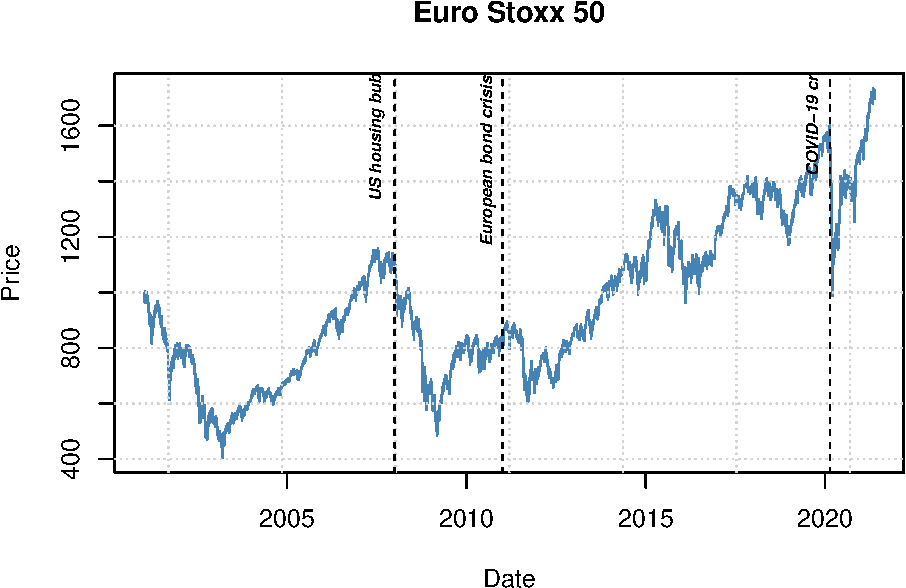
\includegraphics{03-Data-meth_files/figure-latex/plot1-1.pdf} 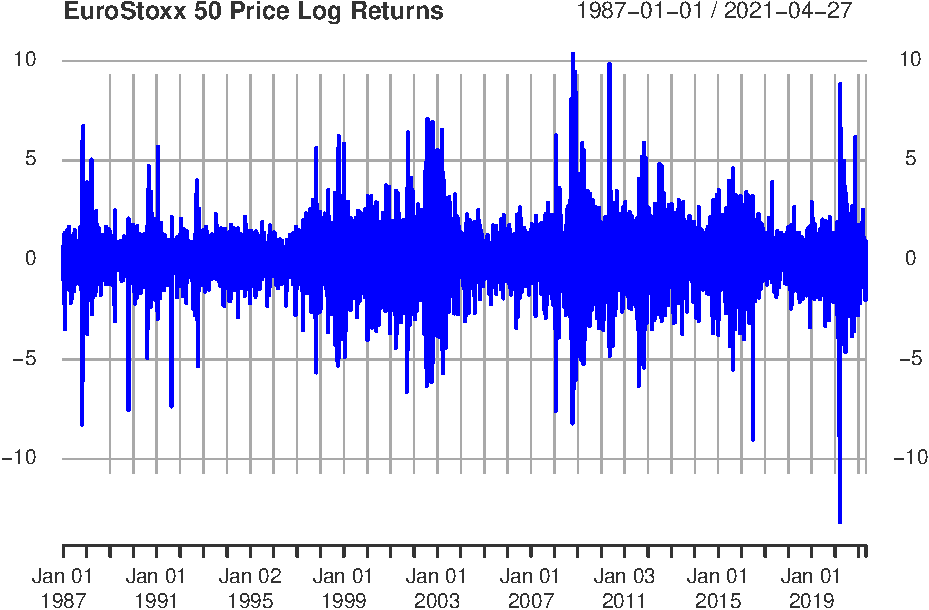
\includegraphics{03-Data-meth_files/figure-latex/plot1-2.pdf}

\begin{figure}
\subfloat[This figure plots the price and price log return respectively for the EuroStoxx 50 index\label{fig:plot2-1}]{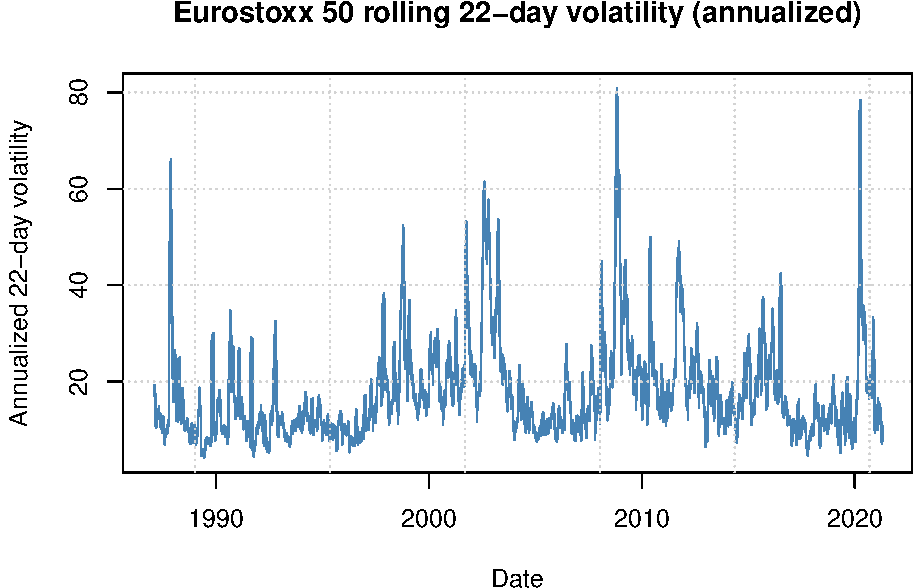
\includegraphics{03-Data-meth_files/figure-latex/plot2-1} }\subfloat[This figure plots the price and price log return respectively for the EuroStoxx 50 index\label{fig:plot2-2}]{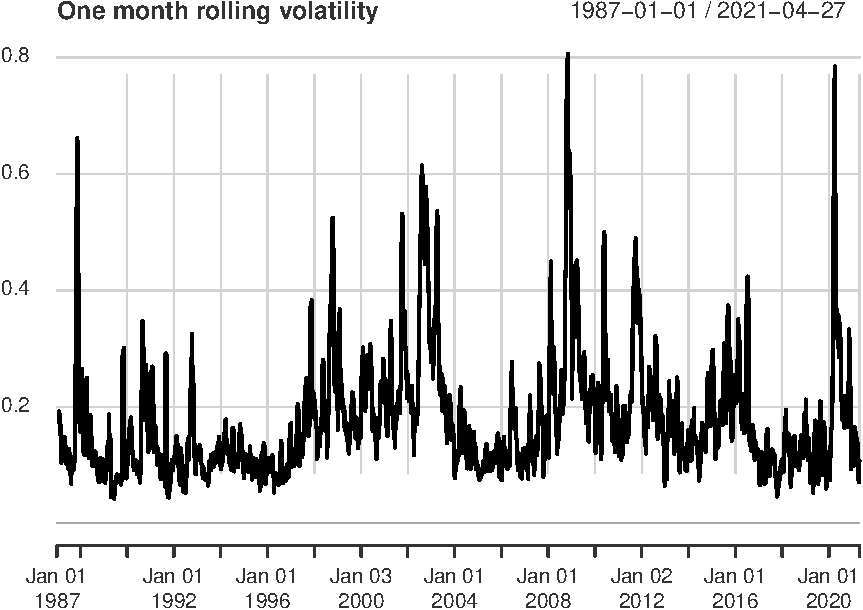
\includegraphics{03-Data-meth_files/figure-latex/plot2-2} }\caption{EuroStoxx 50 price and price log return evolution}\label{fig:plot2}
\end{figure}

As can be seen

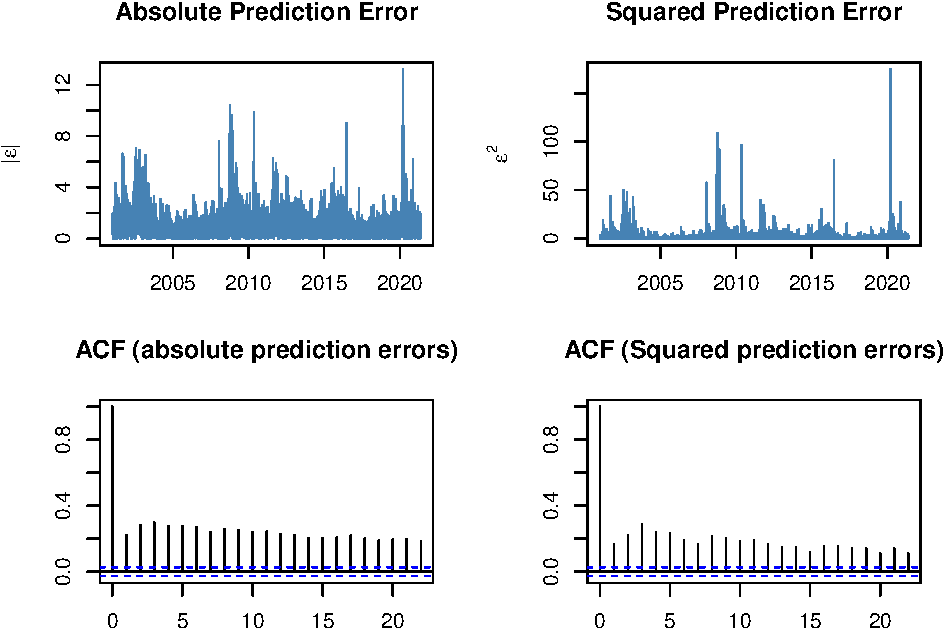
\includegraphics{03-Data-meth_files/figure-latex/acfplots-1.pdf}

\begin{Shaded}
\begin{Highlighting}[]
\NormalTok{distributions }\OtherTok{\textless{}{-}} \FunctionTok{c}\NormalTok{(}\StringTok{"norm"}\NormalTok{, }\StringTok{"snorm"}\NormalTok{, }\StringTok{"std"}\NormalTok{, }\StringTok{"sstd"}\NormalTok{, }\StringTok{"sged"}\NormalTok{)}
\NormalTok{garchspec }\OtherTok{\textless{}{-}}\NormalTok{ garchfit }\OtherTok{\textless{}{-}}\NormalTok{ garchforecast }\OtherTok{\textless{}{-}}\NormalTok{ stdret }\OtherTok{\textless{}{-}} \FunctionTok{vector}\NormalTok{(}\AttributeTok{mode =} \StringTok{"list"}\NormalTok{, }\AttributeTok{length =} \FunctionTok{length}\NormalTok{(distributions))}

\ControlFlowTok{for}\NormalTok{(i }\ControlFlowTok{in} \DecValTok{1}\SpecialCharTok{:}\FunctionTok{length}\NormalTok{(distributions))\{}
\CommentTok{\# Specify a GARCH model with constant mean}
\NormalTok{garchspec[[i]] }\OtherTok{\textless{}{-}} \FunctionTok{ugarchspec}\NormalTok{(}\AttributeTok{mean.model =} \FunctionTok{list}\NormalTok{(}\AttributeTok{armaOrder =} \FunctionTok{c}\NormalTok{(}\DecValTok{0}\NormalTok{,}\DecValTok{0}\NormalTok{)),}
                     \AttributeTok{variance.model =} \FunctionTok{list}\NormalTok{(}\AttributeTok{model =} \StringTok{"sGARCH"}\NormalTok{, }\AttributeTok{variance.targeting =}\NormalTok{ T), }
                     \AttributeTok{distribution.model =}\NormalTok{ distributions[i])}
\CommentTok{\# Estimate the model}
\NormalTok{garchfit[[i]] }\OtherTok{\textless{}{-}} \FunctionTok{ugarchfit}\NormalTok{(}\AttributeTok{data =}\NormalTok{ R, }\AttributeTok{spec =}\NormalTok{ garchspec[[i]])}

\CommentTok{\# Compute stdret using residuals()}
\NormalTok{stdret[[i]] }\OtherTok{\textless{}{-}} \FunctionTok{residuals}\NormalTok{(garchfit[[i]], }\AttributeTok{standardize =} \ConstantTok{TRUE}\NormalTok{)}

\CommentTok{\# Compute stdret using fitted() and sigma()}
\NormalTok{stdret[[i]] }\OtherTok{\textless{}{-}}\NormalTok{ (R }\SpecialCharTok{{-}} \FunctionTok{fitted}\NormalTok{(garchfit[[i]])) }\SpecialCharTok{/} \FunctionTok{sigma}\NormalTok{(garchfit[[i]]) }

\NormalTok{\}}


\CommentTok{\# \# Use the method sigma to retrieve the estimated volatilities }
\CommentTok{\# garchvol \textless{}{-} sigma(garchfit) }
\CommentTok{\# }
\CommentTok{\# \# Plot the volatility for 2017}
\CommentTok{\# plot(garchvol)}
\CommentTok{\# }
\CommentTok{\# \# Compute unconditional volatility}
\CommentTok{\# sqrt(uncvariance(garchfit))}
\CommentTok{\# }
\CommentTok{\# \# Print last 10 ones in garchvol}
\CommentTok{\# tail(garchvol, 10)}

\CommentTok{\# \# Forecast volatility 5 days ahead and add }
\CommentTok{\# garchforecast \textless{}{-} ugarchforecast(fitORspec = garchfit, }
\CommentTok{\#                      n.ahead = 5)}
\CommentTok{\# }
\CommentTok{\# \# Extract the predicted volatilities and print them}
\CommentTok{\# print(sigma(garchforecast))}




\CommentTok{\# \# Compute stdret using residuals()}
\CommentTok{\# stdret[[i]] \textless{}{-} residuals(garchfit[[i]], standardize = TRUE)}
\CommentTok{\# }
\CommentTok{\# \# Compute stdret using fitted() and sigma()}
\CommentTok{\# stdret[[i]] \textless{}{-} (R {-} fitted(garchfit[[i]])) / sigma(garchfit[[i]])}






\CommentTok{\#  make the histogram}

\FunctionTok{chart.Histogram}\NormalTok{(stdret[[}\DecValTok{1}\NormalTok{]], }\AttributeTok{methods =} \FunctionTok{c}\NormalTok{(}\StringTok{"add.normal"}\NormalTok{,}\StringTok{"add.density"}\NormalTok{ ), }
                \AttributeTok{colorset =} \FunctionTok{c}\NormalTok{(}\StringTok{"gray"}\NormalTok{,}\StringTok{"red"}\NormalTok{,}\StringTok{"blue"}\NormalTok{))}
\end{Highlighting}
\end{Shaded}

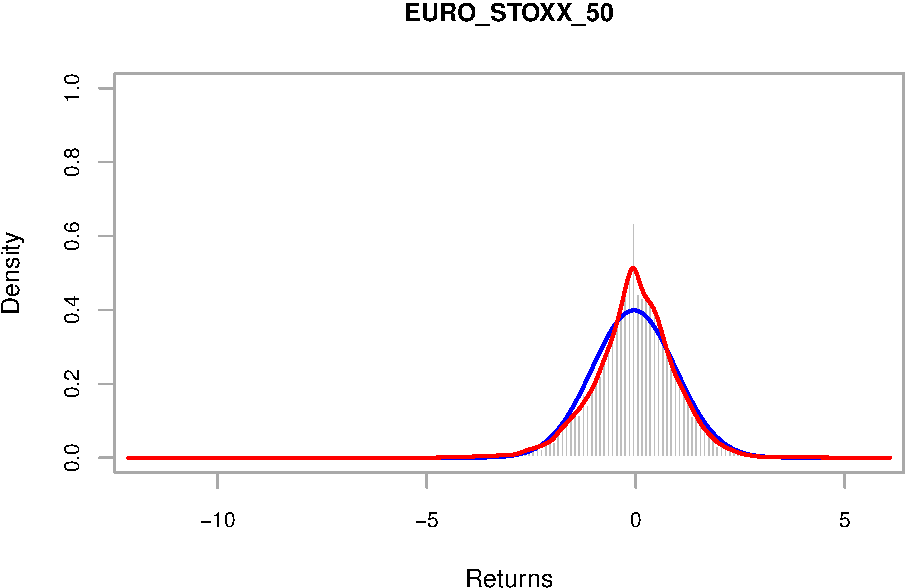
\includegraphics{03-Data-meth_files/figure-latex/unnamed-chunk-1-1.pdf}

\newpage

\hypertarget{methodology}{%
\subsection{Methodology}\label{methodology}}

Here comes text\ldots{}

As already mentioned in \ldots, GARCH models sGARCH, eGARCH, iGARCH, gjrGARCH, nGARCH, tGARCH and tsGARCH will be estimated. Additionally the distributions will be examined as well, including the normal, student-t distribution, skewed student-t distribution, generalised error distribution, skewed generalised error distribution and the skewed generalised Theodossiou distribution.

They will be estimated using maximum likelyhood. As already mentioned, fortunately, Alexios \textcite{alexios2020} has made it easy for us to implement this methodology in R (version 3.6.1) with the package rugarch version 1.4-4 (R univariate garch), which gives us a bit more time to focus on the results and the interpretation.

\clearpage

Let's add an image:

\begin{Shaded}
\begin{Highlighting}[]
\CommentTok{\# knitr::include\_graphics("figures/sample{-}content/captain.jpeg")}
\end{Highlighting}
\end{Shaded}



%%%%% REFERENCES

% JEM: Quote for the top of references (just like a chapter quote if you're using them).  Comment to skip.
% \begin{savequote}[8cm]
% The first kind of intellectual and artistic personality belongs to the hedgehogs, the second to the foxes \dots
%   \qauthor{--- Sir Isaiah Berlin \cite{berlin_hedgehog_2013}}
% \end{savequote}

\setlength{\baselineskip}{0pt} % JEM: Single-space References

{\renewcommand*\MakeUppercase[1]{#1}%
\printbibliography[heading=bibintoc,title={\bibtitle}]}

\end{document}
